% Created 2026-01-03 sáb 13:07
% Intended LaTeX compiler: pdflatex
\documentclass[a4paper]{article}
\usepackage[utf8]{inputenc}
\usepackage[T1]{fontenc}
\usepackage{graphicx}
\usepackage{longtable}
\usepackage{wrapfig}
\usepackage{rotating}
\usepackage[normalem]{ulem}
\usepackage{amsmath}
\usepackage{amssymb}
\usepackage{capt-of}
\usepackage{hyperref}
\usepackage{color}
\usepackage{listings}
\usepackage[spanish]{babel}
\usepackage[usenames,dvipsnames]{color} % Required for custom colors
\renewcommand{\ttdefault}{pcr} % MONOESPACIO CON NEGRIT
\usepackage{lastpage}
\usepackage{listings}
\usepackage{listingsutf8}
\renewcommand{\lstlistingname}{Listado}
\lstset{frame=single,inputencoding=utf8,basicstyle=\scriptsize\ttfamily,showstringspaces=false,numbers=none}
\definecolor{MyDarkGreen}{rgb}{0.0,0.4,0.0} % This is the color used for comments
\lstset{ breaklines=true, postbreak=\mbox{\textcolor{red}{$\hookrightarrow$}\space}, keywordstyle=\bfseries, keywordstyle=[1]\color{Blue}\bfseries,  keywordstyle=[2]\color{Purple}\bfseries,  keywordstyle=[3]\color{Blue}\underbar,   identifierstyle=,   commentstyle=\usefont{T1}{pcr}{m}{sl}\color{MyDarkGreen}\small,   stringstyle=\color{Purple},   showstringspaces=false,   tabsize=2,   morecomment=[l][\color{Blue}]{...} }
\lstset{literate=  {á}{{\'a}}1 {é}{{\'e}}1 {í}{{\'i}}1 {ó}{{\'o}}1 {ú}{{\'u}}1   {Á}{{\'A}}1 {É}{{\'E}}1 {Í}{{\'I}}1 {Ó}{{\'O}}1 {Ú}{{\'U}}1   {à}{{\`a}}1 {è}{{\`e}}1 {ì}{{\`i}}1 {ò}{{\`o}}1 {ù}{{\`u}}1   {À}{{\`A}}1 {È}{{\'E}}1 {Ì}{{\`I}}1 {Ò}{{\`O}}1 {Ù}{{\`U}}1   {ä}{{\"a}}1 {ë}{{\"e}}1 {ï}{{\"i}}1 {ö}{{\"o}}1 {ü}{{\"u}}1   {Ä}{{\"A}}1 {Ë}{{\"E}}1 {Ï}{{\"I}}1 {Ö}{{\"O}}1 {Ü}{{\"U}}1   {â}{{\^a}}1 {ê}{{\^e}}1 {î}{{\^i}}1 {ô}{{\^o}}1 {û}{{\^u}}1   {Â}{{\^A}}1 {Ê}{{\^E}}1 {Î}{{\^I}}1 {Ô}{{\^O}}1 {Û}{{\^U}}1   {œ}{{\oe}}1 {Œ}{{\OE}}1 {æ}{{\ae}}1 {Æ}{{\AE}}1 {ß}{{\ss}}1   {ű}{{\H{u}}}1 {Ű}{{\H{U}}}1 {ő}{{\H{o}}}1 {Ő}{{\H{O}}}1   {ç}{{\c c}}1 {Ç}{{\c C}}1 {ø}{{\o}}1 {å}{{\r a}}1 {Å}{{\r A}}1   {€}{{\euro}}1 {£}{{\pounds}}1 {«}{{\guillemotleft}}1   {»}{{\guillemotright}}1 {ñ}{{\~n}}1 {Ñ}{{\~N}}1 {¿}{{?`}}1 }
\usepackage{caption}
\usepackage{attachfile2}
\usepackage[margin=1.5cm,includeheadfoot,includehead,includefoot]{geometry}
\hypersetup{colorlinks,linkcolor=black}
\usepackage{fancyhdr}
\pagestyle{fancyplain}
\chead{}
\lhead{}
\rhead{}
\cfoot{}
\lfoot{\begin{footnotesize}alvaro.gonzalezsotillo@educa.madrid.org\end{footnotesize}}
\rfoot{\begin{footnotesize}\thepage / \pageref{LastPage}\end{footnotesize}}
\usepackage[skins]{tcolorbox}
\usepackage{multicol}
\usepackage{changepage} %ajdustwidth
\usepackage{fancybox}
\usepackage{attachfile2}
\lhead{Extraordinaria 2021 (es el \\lhead)}
\rhead{Administración y Gestión de Bases de Datos (es el \\rhead)}
\lhead{Git}
\rhead{Entornos de desarrollo}
\usepackage{svg}
\usepackage{letltxmacro}
\LetLtxMacro{\originalincludegraphics}{\includegraphics}
\renewcommand{\includegraphics}[2][]{\IfFileExists{#2.pdf}{\originalincludegraphics[#1]{#2.pdf}}{\originalincludegraphics[#1]{#2}}}
\LetLtxMacro{\originalincludesvg}{\includesvg}
\renewcommand{\includesvg}[2][]{\IfFileExists{#2.pdf}{\originalincludegraphics[#1]{#2.pdf}}{\originalincludegraphics[#1]{#2.svg.pdf}}}
\usepackage{comment}
\excludecomment{NOTES}
\date{}
\title{}
\hypersetup{
 pdfauthor={Álvaro González Sotillo},
 pdftitle={},
 pdfkeywords={},
 pdfsubject={},
 pdfcreator={Emacs 30.2 (Org mode 9.7.11)}, 
 pdflang={Spanish}}
\begin{document}

\captionsetup{font=scriptsize}

\textattachfile{/datos-luks/datos-alvaro/apuntes-clase/entornos-de-desarrollo/apuntes/3/ED-03-practica-git.org}{} \vspace{-1em}


\setlength{\parindent}{0em}
\setlength{\parskip}{1em}

\newtcolorbox{Aviso}[1][Aviso]{
  enhanced,
  colback=gray!5!white,
  colframe=gray!75!black,fonttitle=\bfseries,
  colbacktitle=gray!85!black,
  attach boxed title to top left={yshift=-2mm,xshift=2mm},
  title=#1
}

\newtcolorbox{cuadrito}[1][Ignorado]{
  %drop shadow southeast,
  enhanced jigsaw,
  colback=white,
}


\newcommand{\StudentData}{
  \begin{cuadrito}[1\textwidth]
    \vspace{0.3cm}
    \large{
      \textbf{Apellidos:} \hrulefill \\
      \textbf{Nombre:} \hrulefill \\
      \textbf{Fecha:} \hrulefill \hspace{1cm} \textbf{Usuario:} \hrulefill \\
    }
    \vspace{-0.2cm}
  \end{cuadrito}
}

\newcommand{\StudentDataDniFirma}{
  \begin{cuadrito}[1\textwidth]
    \vspace{0.3cm}
    \large{
      \textbf{Apellidos:} \hrulefill \\
      \textbf{Nombre:} \hrulefill  \\
      \textbf{Dni:} \hrulefill \hspace{8cm} \\
      \\
      \textbf{Firma:} \hrulefill \hspace{8cm} \\
    }
    \vspace{-0.2cm}
  \end{cuadrito}
}
\section{Objetivo de la práctica}
\label{sec:org0000000}
En esta práctica el alumno manejará un repositorio Git, trabajando los siguientes aspectos
\begin{itemize}
\item Uso básico desde línea de comandos o IDE
\item Manejo de diferentes ramas
\item Trabajo colaborativo
\item Corresponden con los CE f) y h) del RA04
\end{itemize}

La última versión de este documento está accesible en \href{https://alvarogonzalezsotillo.github.io/apuntes-clase/entornos-de-desarrollo/apuntes/3/ED-03-practica-git.pdf}{este enlace}
\section{Cuenta en Codeberg}
\label{sec:org0000003}
\begin{enumerate}
\item Crea una cuenta en \href{https://codeberg.org/}{codeberg}. Utiliza tu correo de educamadrid.
\item La práctica se realiza por parejas. En caso necesario, puede haber grupos de tres alumnos.
\item Haz un \emph{fork} del repositorio \url{https://codeberg.org/alvarogonzalezsotillo/Java-Games.git}
\item El repositorio debe ser privado
\begin{itemize}
\item Da permisos completos al profesor alvaro.gonzalezsotillo@educa.madrid.org
\item Da permisos completos a tu compañero de práctica
\end{itemize}
\item Añade el repositorio de tu compañero como un \emph{remote} más de tu proyecto Git
\end{enumerate}
\section{Ramas concurrentes de desarrollo}
\label{sec:org000000f}
Los siguientes trabajos se repartirán entre los integrantes del equipo, de forma concurrente

\begin{multicols}{3}
\subsection{Rama \texttt{translate}}
\label{sec:org0000006}
\begin{itemize}
\item Crea la rama \texttt{translate} a partir de \texttt{master}
\item Traduce a otro idioma las interfaces de los juegos:
\begin{itemize}
\item Tetris
\item MathHero
\item FallDown
\end{itemize}
\end{itemize}
\subsection{Rama \texttt{mainmenu}}
\label{sec:org0000009}
\begin{itemize}
\item Crea la rama \texttt{mainmenu} a partir de \texttt{master}
\item Añade un módulo que implemente un menú para ejecutar cualquier juego
\end{itemize}
\subsection{Rama \texttt{falldownwidth}}
\label{sec:org000000c}
\begin{itemize}
\item Crea la rama \texttt{falldonwwidth} a partir de \texttt{master}
\item Crea una nueva clase de nombre \texttt{PlayFallDownWide} en el módulo \texttt{FallDown}
\item Ejecutará el juego, pero con un tablero el doble de ancho que \texttt{PlayFallDown}
\end{itemize}

\end{multicols}

\begin{figure}[htbp]
\centering
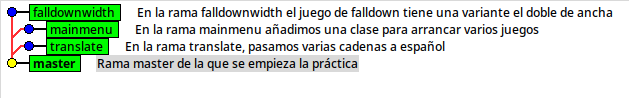
\includegraphics[width=.9\linewidth]{media/practica-todas-las-ramas.png}
\caption{Cómo se ven las ramas en Gitk}
\end{figure}
\section{Fusiones hasta \texttt{master}}
\label{sec:org0000012}
\begin{itemize}
\item Fusiona \texttt{translate} con \texttt{master}
\item Fusiona \texttt{falldownwidth} con \texttt{mainmenu}. El menú debe tener dos entradas para el juego FallDown, una para el juego original y otra para la variante ancha
\item Fusiona \texttt{mainmenu} con \texttt{master}
\end{itemize}
\section{Haz una \emph{release}}
\label{sec:org0000015}
\begin{itemize}
\item Crea una etiqueta (\emph{tag}) con el nombre \texttt{entrega-practica} en la rama \texttt{master} cuando estén todas las ramas fusionadas
\end{itemize}


\begin{figure}[htbp]
\centering
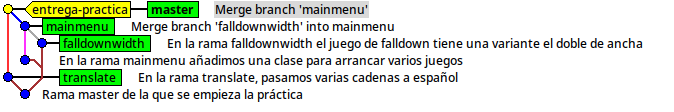
\includegraphics[width=.9\linewidth]{media/practica-todas-las-ramas-fusionadas.png}
\caption{Cómo se ven las ramas ya fusionadas en Gitk}
\end{figure}

\begin{figure}[htbp]
\centering
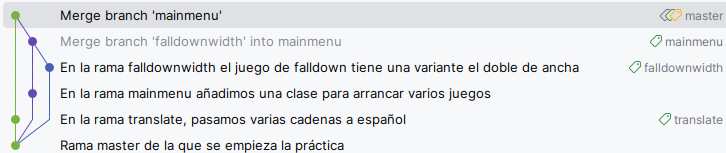
\includegraphics[width=.9\linewidth]{media/practica-todas-las-ramas-fusionadas-intellij.png}
\caption{Cómo se ven las ramas ya fusionadas en Intellij}
\end{figure}

\begin{Aviso}
Dependiendo del orden en que se fusionen las ramas, y de los \emph{commits} intermedios, puede haber diferencias en la visualización de todas las ramas fusionadas
\end{Aviso}
\section{Qué se entrega}
\label{sec:org0000018}
\begin{itemize}
\item Sube en la tarea del aula virtual
\begin{itemize}
\item La URL a tu repositorio. Contendrá todas las ramas, \emph{commits} y etiquetas que se hayan hecho en la práctica (sean propias o de los compañeros)
\item El \emph{hash} del \emph{commit} de la etiqueta \texttt{entrega-practica}
\item La salida del comando \texttt{git log -{}-{}all -{}-{}graph}
\end{itemize}
\end{itemize}
\end{document}
